\documentclass[
	parspace, % Térköz bekezdések közé / Add vertical space between paragraphs
	%noindent, % Bekezdésének első sora ne legyen behúzva / No indentation of first lines in each paragraph
	%nohyp, % Szavak sorvégi elválasztásának tiltása / No hyphenation of words
	%twoside, % Kétoldalas nyomtatás / Double sided format
	%draft, % Gyorsabb fordítás ábrák rajzolása nélkül / Quicker draft compilation without rendering images
	%final, % Teendők elrejtése / Set final to hide todos
]{elteikthesis}[2020/11/23]

% Dolgozat metaadatai
% Document's metadata
\title{Multimédia Vizualizációs Platform} % cím / title
\date{2021} % védés éve / year of defense

% Szerző metaadatai
% Author's metadata
\author{Tarjáni Martin Dominik}
\neptun{FAZMVB}
\degree{Programtervező informatikus BSc}
\educationtype{Nappali}

% Témavezető(k) metaadatai
% Superivsor(s)' metadata
\supervisor{Tarcsi Ádám} % belső témavezető neve / internal supervisor's name
\affiliation{Egyetemi tanársegéd} % belső témavezető beosztása / internal supervisor's affiliation
%\extsupervisor{Külső Kornél} % külső témavezető neve / external supervisor's name
%\extaffiliation{informatikai igazgató} % külső témavezető beosztása / external supervisor's affiliation

% Egyetem metaadatai
% University's metadata
\university{Eötvös Loránd Tudományegyetem} % egyetem neve / university's name
\faculty{Informatikai Kar} % kar neve / faculty's name
\department{Adattudományi és Adattechnológiai \\ Tanszék} % tanszék neve / department's name
\city{Budapest} % város / city
\logo{elte_cimer/elte_cimer_szines} % logo

% Irodalomjegyzék hozzáadása
% Add bibliography file
\addbibresource{thesis.bib}

% A dolgozat
% The document
\begin{document}

% Nyelv kiválasztása
% Set document language
\documentlang{magyar}
%\documentlang{english}

% Teendők listája (final dokumentumban nincs)
% List of todos (not in the final document)
%\listoftodos[\todolabel]

% Dokumentum beállítások
% Some document settings
% Lábjegyzet folytonos számozása fejezetek között
% Continuous counting of footnotes among chapters
\counterwithout{footnote}{chapter}

% Tartalomjegyzék oldalszámozásának rejtése
% Hide page numbering of ToC
\newcounter{conpageno}
\let\oldtableofcontents\tableofcontents
\renewcommand{\tableofcontents}{
	\pagenumbering{gobble}
	\oldtableofcontents
	\cleardoublepage
	\setcounter{conpageno}{\value{page}}
	\pagenumbering{arabic}
	\setcounter{page}{\value{conpageno}}
}


% Címlap (kötelező)
% Title page (mandatory)
\maketitle
%\topicdeclaration

% Témabejelentő (kötelező)
% Thesis Proposal (mandatory)
% Témabejelentő
% Thesis Proposal

\thispagestyle{empty}
{\bf \huge {Szakdolgozati témabejelentő}}

\begin{flushleft}
    {\bf {Hallgató adatai:}}\\
    \> \> \> \> {\emph {Név: }} \authorname\\
    \> \> \> \> {\emph {Neptun kód: }} \neptuncode\\
    \vspace{0.3cm}

    {\bf {Képzési adatok:}}\\
    \> \> \> \> {\emph {Szak: }} \degreename\\
    \> \> \> \> {\emph {Tagozat: }} \studytype\\
    \vspace{0.3cm}

    {\bf {Témavezető neve:}} \supname\\
    \> \> \> \> {\emph {Munkahelyének neve, tanszéke: }}\\
    \> \> \> \> \> \> \> \> {\small {ELTE Informatikai Kar, Adattudományi és Adattechnológiai Tanszék}}\\
    \> \> \> \> {\emph {Munkahelyének címe: }}\\
    \> \> \> \> \> \> \> \> {\small {117 Budapest, Pázmány Péter sétány 1/C., 2. emelet, 2.420-as szoba}}\\
    \> \> \> \> {\emph {Beosztás és iskolai végzettsége: }} \\
    \> \> \> \> \> \> \> \> {\small \supaff}\\
\end{flushleft}

\vspace{0.5cm}

{\bf {A szakdolgozat címe:}} {Multimédia Vizualizációs Platform}\\
\vspace{1cm}
\> \> {\bf {A szakdolgozat témája:}}

A Multimédia Vizualizációs Platform egy számítógépre, külső HDD-re, SSD-re vagy Pendrive-ra letöltött multimédia - főleg filmek, sorozatok - vizualizációjára szolgál, tehát ezen tartalmak fogyasztására egy áttekinthető és könnyen kezelhető felületet biztosít. Hasonlót, amelyhez már hozzászokhattunk a különböző streaming szolgáltatóktól, csak mindezt nem egy külső adatbázisból betöltve, hanem a saját offline tartalmainkra építve. A felület biztosítja az alapvető funkcionalitásokat amelyeket egy videó lejátszó platformtól el lehet várni: filmek listázása, keresés, lejátszás, megállítás, előre-hátra pörgetés, nyelv és felirat választás, lejátszási listák létrehozása stb. Külön kezeli az egyrészes filmek, a több részes filmsorozatok és a több részes TV sorozatok felületeit. A filmekhez és sorozatokhoz továbbá meta-adatokat (Cím, Szereplők, Leírás, Műfajok stb.) tölt le/be, ezzel is növelve a felhasználói élményt.

\vfill

{\it {Budapest}, {2020.12.01.}}

\cleardoublepage

% Köszönetnyilvánítás
% Acknowledgments
% Köszönetnyilvánítás
% Acknowledgments

\thispagestyle{empty}

\vspace*{\fill}

{\bf \huge {Köszönetnyilvánítás}}

\vspace*{\fill}

Soha nem gondoltam volna, hogy ilyen gyorsan eltelnek az egyetemi évek, sok minden történt ezalatt a 4 év alatt és túl hosszú lenne a lista, hogy kiknek is köszönhetek rengeteg mindent. Ennek ellenére megpróbálkozok vele.

Köszönöm a témavezetőmnek, Tarcsi Ádámnak, hogy mindig ott volt amikor kérdésem volt és segített bármiben amiben csak kellett.
Köszönöm Thornak vagyis Gerely Viktor Andrásnak a sok tanácsadást és támogatást amit nyújtott közel se csak a szakdolgozatom elkészültében, de mind a 4 év alatt. Továbbá külön köszönöm a gyönyörű ikon grafikát amit az alkalmazásomhoz készített.
Köszönöm barátaimnak, Vida Bálintnak, Tompa Gábornak és Fenyvesi Leventének, hogy mellettem álltak a legelejétől, a Gólyatábortól kezdve egészen a Záróvizsgáig és azon túl.
Köszönöm oktatóimnak, gyakorlat vezetőimnek, akik szakértelmükkel hozzájárultak, hogy tudásom ezalatt a 4 év alatt exponenciálisan növekedjen.

Végül, de nagyon nem utolsó sorban köszönöm barátnőmnek, Tamás Laurának és szüleimnek a rengeteg támogatást, akik az elejétől fogva támogatnak és mellettem állnak és akik nélkül egészen biztosan nem állhatnék itt ma.

\vspace*{\fill}
% \setcounter{page}{1}

\cleardoublepage

% Tartalomjegyzék (kötelező)
% Table of contents (mandatory)
\tableofcontents
\cleardoublepage

% Tartalom
% Main content
\chapter{Bevezetés} % Introduction
\label{ch:intro}

A mai világban elég hálás dolog film- és sorozat rajongónak lenni, rengeteg tartalommal bombáznak minket a különböző streaming platformok (Netflix, HBO GO), TV csatornák, Youtube csatornák és még sorolhatnánk. Mindazonáltal természetesen semmi sem tökéletes: biztos a Kedves Olvasó is tapasztalta már, hogy kereste a kedvenc filmjét, sorozatát az éppen aktuálisan előfizetett platformon vagy TV-ben. Azonban szinte törvényszerű, hogy amit éppen akarunk nézni az sosincs fent a kínálatban, vagy még rosszabb, amikor fent van, de nem olyan formában, ahogy nekünk az megfelelő (például nincs magyar vagy angol szinkron, magyar felirat stb.).

Mindeközben polcainkon egyre porosodnak - vagy már réges-régen lekerültek onnan - a nem használt CD, DVD és Blu-Ray lemezek és így 2021-ben elérkeztünk oda is, hogy a nagy becsben tartott kedvenc filmjeinket tartalmazó több terrabájtos külső merevlemezünk is a por és a feledés martalékává válik.

Téma választásomat és motivációmat, tehát ezen téma ihlette meg leginkább, hiszen hasonló cipőben járok jómagam is. Temérdek kedvenc filmemnek szerettem volna egy átlátható és szép környezetet biztosítani, amelyen ezen tartalmak fogyasztása még nagyobb élmény.

Alkalmazásommal ezekre a problémákra szeretnék megoldást nyújtani: egy offline tartalmakra, tehát külső meghajtón, SSD-n vagy pendrive-on tárolt és ezekre a tartalmakra épülő, megjelenésében és funkcióiban a már megszokott streaming szolgáltatókra hasonlító, könnyen kezelhető és áttekinthető platform létrehozása.\\
Ez a Multimédia Vizualizációs Platform vagy röviden MVP.

Funkcióit tekintve biztosít mindent, amit egy videó lejátszó platformtól el lehet várni:
\begin{itemize}
    \item Elemek listázása
    \item Keresés
	\item Filmek, sorozatok lejátszása, megállítása
	\item Előre-hátra pörgetés
	\item Felirat választás
	\item Lejátszási listák létrehozása
	\item Külön kezeli a filmek és a több részes sorozatok felületeit
	\item Metaadatok betöltése fájlnévből és NFO fájlból
	\item Metaadatok letöltése TMDB adatbázisból
\end{itemize}


\cleardoublepage

\chapter{Felhasználói dokumentáció} % User guide
\label{ch:user}

\section{TODO}
\subsection{Tartalom}
\begin{itemize}
    \item megoldott probléma rövid megfogalmazása
	\item felhasznált módszerek rövid leírása
	\item program használatához szükséges összes információ, gépigény, telepítés, futtatás
	\item alkalmazás bemutatása hogy az átlag felhasználó megértse
	\item képernyőképek amik segítik a program használatát
	\item use-case-ek használata amivel bemutatom a funkciókat
\end{itemize}

\subsection{Bírálati szempontok}
Magába foglalja a telepítési- (vagy üzemeltetési-) és a végfelhasználói leírást. Ezek meghatározott célközönséghez szólnak, könnyen és gyorsan kell, hogy eligazítsák a felhasználót a program használatában!
Tartalma:
\begin{itemize}
    \item A feladat rövid ismertetése (mire való a szoftver)
	\item Célközönség (kik, mikor, mire használhatják a programot)
	\item A rendszer használatához szükséges minimális, illetve optimális HW/SW környezet
    \item Első üzembe helyezés leírása – ha van ilyen –, a program indítása (kivéve, ha nem egy önálló alkalmazásról, hanem egy meglévő rendszer új komponenséről van szó). Itt ellenőrizzük, hogy a telepítési útmutató megfelel-e a valóságos telepítési folyamatnak.
    \item Általános felhasználói tájékoztató (például a szokásostól eltérő képernyő-, billentyű-, illetve egérkezelés leírása, teendők hibaüzenetek esetén stb.).
    \item A rendszer funkcióinak ismertetése. A feladat jellegéből fakadóan célszerű lehet ezt folyamatszerűen, képernyőképekkel alátámasztva bemutatni. A funkciókat ajánlatos a felhasználói szintek szerint csoportosítani. Itt vegyük figyelembe, hogy a leírás a fejlesztői dokumentációban meghatározott részfeladathoz illeszkedik-e, az ott meghatározott funkciókat/használati eseteket írja-e le?
    \item A rendszer futás közbeni üzenetei (hibaüzenetek, figyelmeztető üzenetek, felszólító üze-netek stb.) és azok magyarázata – az esetleges üzemeltetési teendőkkel együtt. Itt vegyük figyelembe, hogy tartalmaz-e biztonsági, illetve hibaelhárítási előírásokat?
    \item Egyéb, a szoftver használatához szükséges információk.

\end{itemize}

\noindent\makebox[\linewidth]{\rule{\paperwidth}{0.4pt}}
% -------------- ITT KEZDŐDIK A LÉNYEGI RÉSZ ------------------------

\cleardoublepage

\chapter{Fejlesztői dokumentáció} % Developer guide
\label{ch:dev}

% ==========================================================
% |     Követelmény specifikáció, Megvalósítás lépései     |
% ==========================================================
\section{Követelmény specifikáció}
Az alkalmazás működéséhez és a feladatleírás teljesítéséhez az alábbi funkciókat kell implementálni:
\begin{itemize}
    \item {\textbf {Film felsoroló platform: }} Az alkalmazásnak felületet kell biztosítania a beolvasott média tartalmak megjelenítéséhez, listázásához.
    \item {\textbf {Média tartalmak beolvasása: }} Mappák kiválasztásával az azokban fellelhető média tartalmak beolvasása.
	\item {\textbf {Keresés a média tartalmak között: }} Az alkalmazásnak lehetőséget kell biztosítania a beolvasott média tartlamak közötti kereséshez.
	\item {\textbf {Lejátszás, Megállítás, Pörgetés: }} Biztosítania kell a videók lejátszását.
	\item {\textbf {Felirat választás: }} Feliratok megjelenítése lejátszáskor, amennyiben elérhető.
	\item {\textbf {Sorozatok és filmek kezelése: }} A felület kezelje külön a sorozatokat és filmeket, tehát például a sorozat epizódjai ne külön-külön jelenjenek meg a listában, hanem a sorozatra rákattintva, annak adatlapján legyenek listázva az epizódok.
	\item {\textbf {Metaadatok betöltése és letöltése: }} Használható és értelmes adatok beolvasása fájlnévből, mappanévből, NFO fájlból és külső adatbázisból metadatokat kell tudnia letölteni.
    \item {\textbf {Lejátszási listák: }} Lehessen lejátszási listákat létrehozni, törölni, ezen listákat filmekkel feltölteni.
\end{itemize}

\section{Megvalósítás lépései}
\begin{enumerate}
    \item {\textbf {Követelmények elemzése: }} Meghatározom az elvégzendő feladatokat a feladatleírás alapján.
    \item {\textbf {Fejlesztési környezetek kiválasztása, megismerése: }} Kiválasztottam, majd elsajátítottam az ismereteket a projekt elvégzéséhez szükséges technológiákból.
    \item {\textbf {Tervezés: }} Megterveztem az alkalmazás alap logikáját, a média tartalmak beolvasását, ezek megjelenítését, a felhasználói felületet.
    \item {\textbf {Adattárolás: }} Az alkalmazáshoz leginkább illő és egyszerű adattárolás kiválasztása, amely lehetőséget biztosít a felhasználói felület dinamikus változásaira: Redux.
    \item {\textbf {Scannelés implementálása: }} Az alkalmazás legfontosabb részének, a média tartalmak beolvasásának megvalósítása.
    \item {\textbf {Felhasználó felület: }} Dizájn megtervezése és a beolvasott adatok helyes megjelenítésének implementálása.
    \item {\textbf {Hátramaradt tervezett és plusz funkciók megvalósítása: }} Például az adatok dinamikus kezelése felhasználó felületről: média törlése, borító hozzáadás, kereső, lejátszási listák stb.
    \item {\textbf {Tesztelés: }} Habár a tesztelés a lista végére került, de a valóságban kézi tesztelés mindegyik lépés végén és közben is megtörtént, a funkciók helyes működésének érdekében. Végezetül a teljes program tesztelése.
\end{enumerate}

% ==========================================================
% |                Használt technológiák                   |
% ==========================================================
\cleardoublepage
\section{Használt technológiák}
Az alkalmazás fejlesztését JavaScript nyelven kezdtem meg és fejlesztés közben váltottam TypeScript nyelvre. A TypeScript gyakorlatilag egy típusos kiterjesztése a JavaScriptnek, éppen ezért minden kód amit JavaScriptben írtam azok érvényes és valid kódok TypeScriptben is. A TypeScript lényege, hogy típus biztossá teszi az alkalmazást, ami ugyan megnehezíti a fejlesztést, de nagy előnye, hogy sok probléma már a fejlesztés során észlelhető - ezáltal javítható - és nem a kész verzióban történnek katasztrofális dolgok. Váltásom motivációja a TypeScript nyújtotta előnyök mellett az is volt, hogy az ipar jelenlegi trendjei teljes egészében efelé a nyelv felé mutatnak, minden komolyan vehető alkalmazás - amely Electront, Angulart vagy más hasonló webes technológiát használ - már TypeScript nyelven íródik. Ez formálta az én hozzáállásomat is a nyelvhez, tekintve, hogy a legelejétől fogva célom volt a legfrissebb és legnépszerűbb technológiák használata, ezen piacképes tudások elsajátítása.

Az alkalmazás fejlesztése teljes egészében a Visual Studio Code nyílt forráskódú kódszerkesztővel zajlott, Electron-t, React-et és Redux-ot továbbá Git verziókezelő rendszert felhasználva és egy publikus GitHub repositoryban tárolva a kódot, amely elérhető az alábbi címen: \url{https://github.com/TMD44/mvp}\cite{github}

\subsection{Electron}
Az Electron\cite{electron} egy nyílt forráskódú keretrendszer, amely asztali alkalmazások fejlesztéséhez lett kifejlesztve. Különlegessége, hogy a már ismert és bejáratott webes technológiákat - tehát HTML, CSS, JavaScript - lehet használni asztali alkalmazások fejlesztéséhez. Az Electron két külön, egymástól hermetikusan elzárt része a {\it main process} és a {\it renderer process}, melyek között alá-fölé rendelt viszony található.

Az Electron ``fő szála'' - ezt nem véletlenül tettem idézőjelbe, tekintve a JavaScript egy egyszálú programozási nyelv, tehát JavaScriptben nem tudunk konkurens programokat írni -, vagy hívhatjuk angolul {\it main process}nek is, ami gyakorlatilag egy Node.JS alkalmazás, amely a böngésző ablakok létrehozásáért, az operációs rendszerrel való kommunikációért és az alkalmazás életciklusáért felel. Ez tulajdonképpen egy fájl, amely az alkalmazásunk belépési pontját fogja képezni.

Az előbb említett böngésző ablak pedig az Electron másik elszeparált és alárendelt része, a {\it renderer process}, amelyet a {\it main process} hoz létre és menedzseli is azt. Ez tulajdonképpen egy Chromium böngésző ablakot jelent, amely egy HTML fájlt fog megjeleníteni, ahogy azt a webes világban már megszokhattuk. Lehetőgésünk van továbbá Node integrációra is, amit a {\it main process}-en belül tudunk engedélyezni. Az integráció lényege, hogy a böngésző ablakból használhatjuk a Node által nyújtott funkciókat is, például fájlrendszer elérése, modulok importálása és exportálása.

\subsection{React}
A React\cite{react}  egy JavaScript könyvtár, amely főleg felhasználó felületek készítésére nyújt egy fölöttébb elegáns megoldást. A segítségével rendkívül egyszerűen tudunk, úgy nevezett Single Page Application-ket készíteni. Az innováció ebben a megközelítésben az, hogy nincs szükség az oldal újbóli betöltésére, hanem a felhasználói interakció során az oldal tartalmai dinamikusan újratöltődnek és nem is az egész oldal, hanem annak kisebb részei, úgy nevezett komponensei.

\subsection{Redux}
A Redux\cite{redux}  egy state management tool, vagyis magyarul egy állapot kezelő rendszer. A Redux lényege és legnagyobb előnye, hogy az alkalmazásunk állapotát képes egy külön egységként tárolni és menedzselni. Az állapotot a memóriában tárolja, gyakorlatilag egy nagy JSON objektumban, ezen adatok módosítása pedig {\it dispatch} útján valósítható meg.

% ==========================================================
% |               Használati esetek diagram                |
% ==========================================================
\cleardoublepage
\section{Használati esetek diagram}
\begin{figure}[H]
	\centering
	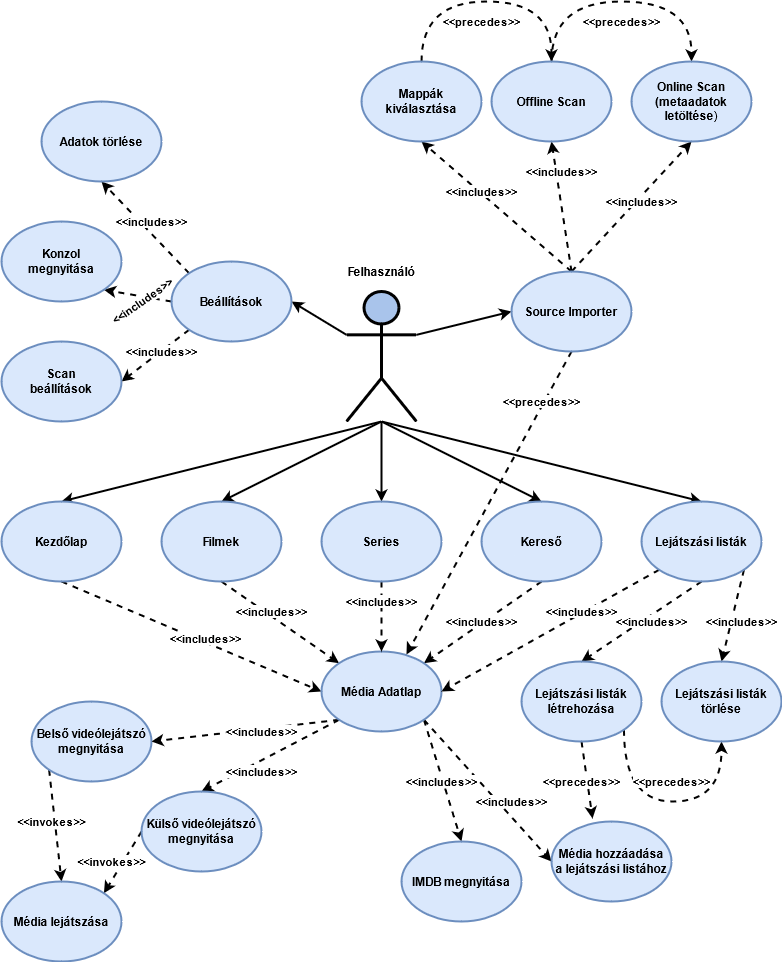
\includegraphics[width=1\textwidth]{use_case_diagram.png}
	\caption{Használati esetek diagram}
	\label{fig:use_case_diagram}
\end{figure}
% \cleardoublepage

% ==========================================================
% |                    Implementáció                       |
% ==========================================================
\section{Implementáció}

\subsection{Mappa struktúra}
\begin{figure}[H]
	\centering
	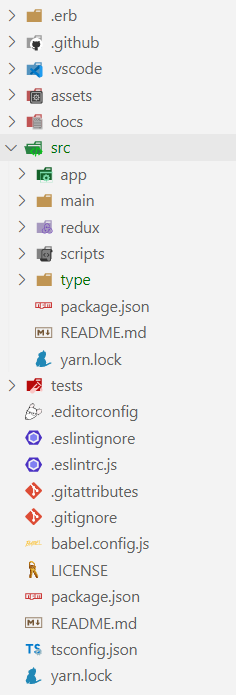
\includegraphics[width=0.3\textwidth]{folders.png}
	\caption{Mappa struktúra}
	\label{fig:folders}
\end{figure}
Az {\it .erb} mappa tartalmazza a Webpack konfigurációkat, illetve olyan eljárásokat, amelyeket sima npm parancsokkal nem lehetne elvégezni. Ezek a fájlok az Electron-React-Boilerplate-ből jönnek, amely egy szabad felhasználású kiindulópontot biztosít az Electron-React alkalmazások számára, én kisebb változtatásokat eszközöltem a saját projektem érdekében.
A {\it .github} és {\it .vscode} mappák csupán konfigurációkat tartalmaznak a GitHub repository, illetve a kódszerkesztő program használatához.
Az {\it .assets} mappa tartalmazza az alkalmazás ikonkészletét, felhasznált képeket, illetve itt kapott helyet a {\it .storage} mappa is, amelyben tárolódik az a két JSON fájl, amelybe az alkalmazás kimenti az adatokat.
Az {\it .docs} mappában a dokumentáció LaTeX-es verziója található.
Az {\it .tests} mappában találhatóak a teszt fájlok.

A {\it .src} mappa pedig az applikáció főkönytára, amelyben helyt kapott az {\it .app} amely a felhasználói felület implementációját és az Electron renderer processét - többek között a Scannelés implementációját is -  tartalmazza, a {\it .main}, amely az Electron main processét tartalmazza, a {\it redux} mappa, amely az adat tároláshoz használt Reduxnak ad helyet. Illetve a {\it scripts} és {\it type} mappák, amely az egész alkalmazásban gyakran használt függvényeket és TypeScript típusokat tartalmazzák.

% ==========================================================
% |               Adatok tárolása, kezelése                |
% ==========================================================
\subsection{Adatok tárolása, kezelése}
Az alkalmazás futása közben a Redux segítségével kezeljük a felhasználói felülethez és a beolvasott média tartalmakhoz kapcsolódó adatokat. Reduxot főleg webalkalmazásokhoz használnak, de nekünk itt asztali környezetben is alkalmazható lesz egy kis trükkel, mégpedig amikor megnyitjuk az alkalmazást, a Redux beállítja a kezdeti állapotot - ez a webes környezetben annyit tenne, hogy egy előre meghatározott alapértelmezett állapot sémát alkalmazna - ami a mi esetünkben két fájl lesz, a {\it config.json} és a {\it mediaDB.json}. A {\it config.json} fájl az alkalmazás futásához, a beolvasáshoz és a felhasználó személyes preferenciáihoz szükséges adatokat, míg a {\it mediaDB.json} fájl a beolvasott média tartalmakhoz kapcsolódó adatokat, metaadatokat tartalmazza. Ez a két JSON fájl kétféleképpen jöhet létre:
\begin{itemize}
    \item Létrejöhet az alkalmazás bezárásakor, ekkor az alkalmazás jelenlegi állapota kerül kiírásra a fájlokba.
    \item Valamint létrejöhet az alkalmazás indításakor is, ha a program úgy érzékeli, hogy a megadott helyen még nem létezik ez a két fájl. Ilyenkor egy előre megadott, alapértelmezett állapot kerül kiírásra, amely alap beállításokat (felhasználói felület, beolvasással kapcsolatos preferenciák stb.) és egy üres vázat tartalmaz, amelybe kerülnek majd a scannelés során gyűjtött adatok.
\end{itemize}

\begin{figure}[H]
	\centering
	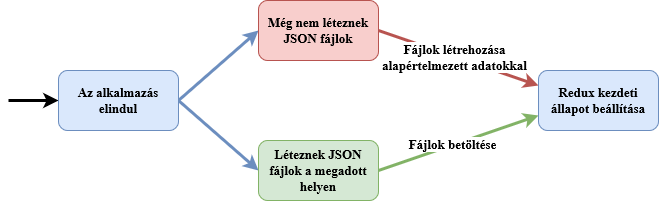
\includegraphics[width=1\textwidth]{Redux_init.png}
	\caption{A Redux kezdeti állapot beállítása}
	\label{fig:redux-init}
\end{figure}

Tehát az alkalmazás futása közben az adatok a Redux storeban tárolódnak, amikor az alkalmazás bezárásra kerül, akkor az állapot két fájlba kerül kiírásra - ebből fakadóan két futás között az adatok fájlban tárolódnak - amit aztán újranyitás esetén egyszerűen betöltünk a kezdeti állapotba.

\subsubsection{Példa config.json fájl}

\lstset{caption={Példa config.json fájl}, label=src:json}
\begin{lstlisting}[language={json}]
{
"creation_time": "2021.05.10. 12:00:00",
"modification_time": "2021.05.10. 12:00:00",
"user_info": { "name": "Anonymous" },
"app_info": {
  "app_name": "Multimedia Visualization Platform",
  "app_version": "0.1.0",
  "app_current_directory": "G:\\mvp\\src\\main",
  "app_locale": "hu",
  "app_locale_country_code": "HU",
  "app_paths": {
    "home": "C:\\Users\\tmd-pc",
    "user_data": "C:\\Users\\tmd-pc\\AppData\\Roaming\\Multimedia Visualization Platform",
    "desktop": "C:\\Users\\tmd-pc\\Desktop",
    "downloads": "C:\\Users\\tmd-pc\\Downloads",
  }
},
"scan_preferences": {
  "scan_language": "en-US",
  "scan_paths": [ "G:\\SOROZATOK" ],
  "scan_file_types": {
    "media": [ ".mkv",".mp4",".avi" ],
    "sub": [ ".srt",".ass",".vtt",".ssa",".sub",".stl",".scc" ],
    "nfo": [ ".nfo" ]
  },
  "scan_results": {
    "media": [{
      "fn": "Game.of.Thrones.S01E01.BDRIP.x264.Hun.Eng",
      "ext": ".mkv",
      "path": "G:\\SOROZATOK\\Game.of.Thrones.COMPLETE.BDRIP.x264.Hun.Eng",
      "full": "G:\\SOROZATOK\\Game.of.Thrones.COMPLETE.BDRIP.x264.Hun.Eng\\Game.of.Thrones.S01E01.BDRIP.x264.Hun.Eng.mkv"
      }],
    "sub": [{
      "fn": "Game.of.Thrones.S01E01.BDRIP.x264.Hun.Eng",
      "ext": ".srt",
      "path": "G:\\SOROZATOK\\Game.of.Thrones.COMPLETE.BDRIP.x264.Hun.Eng",
      "full": "G:\\SOROZATOK\\Game.of.Thrones.COMPLETE.BDRIP.x264.Hun.Eng\\Game.of.Thrones.S01E01.BDRIP.x264.Hun.Eng.srt"
      }],
    "nfo": [{
      "fn": "Game.of.Thrones.COMPLETE.BDRIP.x264.Hun.Eng",
      "ext": ".nfo",
      "path": "G:\\SOROZATOK\\Game.of.Thrones.COMPLETE.BDRIP.x264.Hun.Eng",
      "full": "G:\\SOROZATOK\\Game.of.Thrones.COMPLETE.BDRIP.x264.Hun.Eng\\Game.of.Thrones.COMPLETE.BDRIP.x264.Hun.Eng.nfo"
      }],
  }
}}
\end{lstlisting}

\cleardoublepage
\subsubsection{Példa mediaDB.json fájl}

\lstset{caption={Példa mediaDB.json fájl}, label=src:json}
\begin{lstlisting}[language={json}]
{
"creation_time": "2021.05.09. 14:44:49",
"modification_time": "2021.05.09. 14:44:49",
"movies": {
  "23b5b6d765ac7a28badbd2f6e6d31ea3": {
    "id": [ "23b5b6d765ac7a28badbd2f6e6d31ea3" ],
    "media_type": "movie"
  },
  "6209ef3cb9451c0def78013521b84d5f": {
    "id": [ "6209ef3cb9451c0def78013521b84d5f" ],
    "media_type": "movie"
  },
},
"tv_series": {
  "Game of Thrones": {
    "id": [
      "98cddc3eb8b19c7ebb2a84049c5fc4f0",
      "6a216938ea15d2a1e5282ec47d9a0649",
      "6044b7976f57147dd35da9c3719fd921",
    ],
    "media_type": "series"
  }
},
"playlists": {
  "Favorites": {
    "contents": {
      "Game of Thrones": {
        "id": [
          "98cddc3eb8b19c7ebb2a84049c5fc4f0",
          "6a216938ea15d2a1e5282ec47d9a0649",
          "6044b7976f57147dd35da9c3719fd921",
        ],
        "media_type": "series"
      }
    },
    "media_type": "playlist"
  }
},
"all_media": {
  "98cddc3eb8b19c7ebb2a84049c5fc4f0": {
    "id": "98cddc3eb8b19c7ebb2a84049c5fc4f0",
    "media_name": "Game.of.Thrones.S01E01.BDRIP.x264.Hun.Eng",
    "extension": ".mkv",
    "path": "G:\\SOROZATOK\\Game.of.Thrones.COMPLETE.BDRIP.x264.Hun.Eng",
    "full_path": "G:\\SOROZATOK\\Game.of.Thrones.COMPLETE.BDRIP.x264.Hun.Eng\\Game.of.Thrones.S01E01.BDRIP.x264.Hun.Eng.mkv",
    "subtitles": [ "G:\\SOROZATOK\\Game.of.Thrones.COMPLETE.BDRIP.x264.Hun.Eng\\Game.of.Thrones.S01E01.BDRIP.x264.Hun.Eng.vtt" ],
    "nfo": "G:\\SOROZATOK\\Game.of.Thrones.COMPLETE.BDRIP.x264.Hun.Eng\\Game.of.Thrones.COMPLETE.BDRIP.x264.Hun.Eng.nfo",
    "metadata": {
      "title": "Game of Thrones",
      "season": 1,
      "episode": 1,
      "languages": ["HUN", "ENG"],
      "codec": "X264",
      "quality": "BDRIP",
      "media_type": "series",
      "imdb_id": "tt0944947",
      "imdb_url": "https://www.imdb.com/title/tt0944947"
    }
  },
}}
\end{lstlisting}

% ==========================================================
% |               Média tartalmak beolvasása               |
% ==========================================================
\cleardoublepage
\subsection{Média tartalmak beolvasása}
Az alkalmazás egyértelműen legfontosabb része, a média tartalmak beolvasása. Ezt a folyamatot három részre bontottuk, a mappák kiválasztására, az Offline, illetve Online Scannelésre.

\subsubsection{Mappa kiválasztás}
A mappák megnyitásához az Electron egy beépített modulját, a {\it dialog}ot fogjuk használni. A probléma csak az, hogy ezt a modult nem lehet a renderer processben használni csak a main processben, ilyenkor jön jól az IPC renderer és IPC main modulok amelyek kommunikációt tesznek lehetővé a két réteg között. Az {\it Open Dir} gombra kattintva tehát elküldjük az IPC-n keresztül a main process-nek, ami aztán a {\it dialog} modult felhasználva megnyitja az operációs rendszer natív párbeszédablakát, ebben az esetben kifejezetten mappák megnyitását engedélyezzük csak, azokból is többet. Az ablakot bezárva az eredményt string tömb formájában visszaküldjük a renderer processnek, amely elvégzi a Redux storeba dispatch-elését. A config objektumon belül {\it scan\_paths} kulcs néven találjuk a beolvasott mappák tömbjét.

\lstset{caption={Mappák megnyitása}, label=src:ts}
\begin{lstlisting}[language={ts}]
ipcMainCommunication.on('open-dir-sync', (event) => {
  dialog
    .showOpenDialog(window, {
      properties: ['openDirectory', 'multiSelections'],
    })
    .then((result) => {
      if (result.canceled === false) {
        event.returnValue = result.filePaths;
      } else {
        event.returnValue = [];
      }
    })
    .catch((err) => {
      console.error(err);
    });
});
\end{lstlisting}

\subsubsection{Offline scan}
Az Offline scannelés megkezdéséhez két dologra lesz szükségünk, az egyik a mappák, amelyekben keresni fogunk, a másik, hogy milyen fájl típusokat fogunk keresni, igencsak hatékonytalan lenne, ha minden fájlt beolvasnánk, amelyek a program működését tekintve nem lényeges információkat tartalmaznak, éppen ezért szűrni fogjuk a fájlokat. A Redux storeból tehát behívjuk a {\it scan\_file\_types} kulcshoz tartozó objektumot, amely egy tematikusan tömböket tartalmazó objektum, ezek előre meghatározott fájltípusok, a felhasználónak lehetősége van megváltoztatni őket. Behívjuk továbbá az előző pontban hozzáadott {\it scan\_paths}-eket.

\lstset{caption={Offline scan}, label=src:ts}
\begin{lstlisting}[language={ts}]
const { media, sub, nfo } = getScanFileTypes();
const paths = getScanPaths();
for (const i in paths) {
  const files = await scanDir(paths[i], [media, sub, nfo].flat());
  for (const j in files) {
    if (!excludedFromScan(files[j])) {
      fileSorting(files[j], media, sub, nfo, scanResults);
    }
  }
}

store.dispatch(addScanResults(scanResults));
const results = getScanResults();

for (const file in results.media) {
  const result = await mediaJSONGenerator(
    results.media[file],
    results
  );
  mediaInJSON[result.id] = result;
}
store.dispatch(addMediaAtOnce(mediaInJSON));
\end{lstlisting}

A megadott mappa elérési útvonalakon végig iterálva minden útvonalra meghívjuk a {\it scanDir } függvényt amely rekurzívan a mappa tartalmán - amennyiben a mappában még több mappa található, ezekben az estekben is hasonlóképpen jár el - és a megadott fájltípusokra szűrve egy tömbbe pusholja a talált fájlokat (videófájlok, például {\it .mkv },{\it .mp4 } vagy feliratfájlok, például {\it .srt }, {\it .vtt }, illetve NFO fájlok {\it .nfo }). Történik még egy filterezés ezt követően is, tekintve nagyon sok példa van rá, hogy az offline videó tartalmaink mellet úgynevezett {\it sample } vagy minta videófájlok is helyet kapnak, ezek a fájlok szűrésre kerülnek, ugyanis a program működésének szempontjából lényegtelen fájlokról beszélünk. Ezután minden talált elemet átalakít egy sokkal kezelhetőbb formátumra, a fentebb már config.json példában bemutatott {\it scan\_results} kulcsban. A lényeg itt annyi, hogy a megfelelő formátumú fájlokat a megfelelelő objektumra szortírozzuk, tehát média fájlokat a media objektumba, a feliratfájlokat a sub objektumba, az NFO fájlokat pedig az nfo objektumba. Mindezek elvégzése után elmentjük a Redux storeba megintcsak dispatch útján.

A következő for ciklusban már ezeket az átalakított objektumokat fogjuk felhasználni és tovább alakítjuk  {\it mediaJsonGenerator} függvény segítségével. A függvény először összepárosítja a feliratfájlokat a hozzá kapcsolódó videófájlhoz, tekintve a feliratfájloknál eddig is az volt a konvenció, hogy a feliratfájl neve legyen ugyanaz, mint a videófájl neve, ezt felhasználva könnyű dolgunk van. Végeredményben egy tömböt fogunk kapni, amely tartalmazza a videófájlhoz köthető feliratokat. A feliratfájlokkal történik a program ezen pontján még egy fontos dolog, mégpedig egy {\it .vtt } formátumra konvertálás, ennek oka az, hogy habár asztali alkalmazást készítünk az eszköztár, amelyet használunk webes technológiákra épülnek, éppen ezért igazodnunk kell a web által támogatott formátumokra, amely jelen esetünkben feliratfájlok esetén a {\it .vtt }.

Ezután az NFO fájl - általában egy NFO fájl köthető egy videófájlhoz - videófájlhoz párosítása következik. Ez már kicsit bonyolultabb eset, itt is fenn áll ugyan a ``legyen ugyanaz a neve'', de a fájlstruktúrán belül a fájl elhelyezkedése változhat. Sorozatok esetén például általában nincs mindegyik epizódhoz külön NFO fájl, hanem magához az évadhoz vagy az egész sorozathoz, tehát a fájl helye nem feltétlenül a videófájl mellet található. A scannelés folyamata lekezeli ezeket a különböző eseteket, tehát végeredményben megkapjuk a videófájlhoz köthető NFO fájlt.
Innentől kezdve rendelkezünk tehát NFO fájllal, amely rengeteg hasznos offline információt tartalmaz a filmünkről, azonban itt olyan problémába ütközünk, hogy az NFO fájl tartalmát tekintve semmilyen konvenció vagy szokás nincs, éppen ezért algoritmikus úton kimondottan nehéz biztosan helyes információkat kinyerni. Ennek következtében az NFO fájlban kifejezetten csak a legfontosabb információt fogjuk keresni, mégpedig egy IMDB linket. Az IMDB a legelterjedtebb filmes adatbázisok egyike jelenleg és az url címében a film egy egyedi azonosítója található, amelyet fel fogunk tudni használni majd a metaadatok letöltésekor. Az NFO fájl tartalmának beolvasását követően, egy reguláris kifejezés segítségével IMDB azonosítót keresünk, ha találtunk akkor nincs is más dolgunk mint lementeni egy objektumba, amit aztán visszaadunk a {\it mediaJsonGenerator } függvénynek. Abban az esetben ha nem találtunk explicit azonosítót, megpróbálkozunk másképp.
Számos esetben megfigyelhető, hogy az NFO fájlokban URL rövidítő szolgáltatásokat használnak, például TinyURL, Bit.ly stb. Scannelésünk folyamatában rendkívül fontos információ az IMDB ID, éppen ezért az algoritmus az egyik legnépszerűbb a TinyURL visszafejtésével is megpróbálkozik. Abban az esetben ha sikerrel jár és a rezolválás eredménye egy IMDB azonosító, akkor a már fentebb ismertetett módon járunk el, ha nem járunk sikerrel akkor az információ nem kerül bele az eredmény objektumba.

A másik forrás amelyből offline használható információkat tudunk kinyerni, a fájlnév és a mappa neve. Ehhez a fájlnév felismerő függvényünket fogjuk használni, amely az NFO-s azonosító felismeréshez hasonlóan regulásris kifejezések szövegre illesztésével fogjuk kivitelezni.
Az {\it fnr} függvény a következőképpen működik, megkap egy stringet, ami az egyik esteben a fájl neve, a másik esetben a mappa neve. Ezután sorban reguláris kifejezéseket illeszt a szövegre és ha illeszkedik rá azt a szövegből kivesszük és a visszaadandó eredmény objektumba rakjuk, az eredeti stringben pedig aláhúzás (\_) karakterre cseréljük a talált eredményt. Ezt minden egyes Regex típusra elvégezzük, ennek következtében a végére kapunk egy eredmény objektumot, amelyben tematikusan szét van válogatva a talált stringek, illetve a visszamaradó szöveget, amelyben már valószínűleg csak a cím maradt az egyetlen hasznos információ. Ekkor az algoritmus a string elejétől elkezd ``értelmes karaktereket'' keresni tehát kisbetűs, nagybetűs karakterek illetve számok, és addig megy a szövegben amíg el nem kezd találni minimum kettő vagy annál több ``értelmetlen karaktereket'', ezek az aláhúzás (\_), a pont (.) és a szóköz ( ). Ha kettő vagy több ``értelmetlen karaktert'' találtunk, akkor az addig ``értelmes'' karaktereket kimentjük, ez lesz a cím. Továbbá kicsit szépítünk is rajta például, ha a szavak között pont van azt szóközre cseréljük és az első karaktert is nagybetűsre cseréljük. Abban az esetben ha valami hiba történik a cím keresésekor a string már üres, vagy rossz formátumú, tehát üres stringet adna vissza, az algoritmus az eredeti, még a függvény paraméterül megkapott stringet teszi meg címnek.

\lstset{caption={Példa reguláris kifejezésekre}, label=src:json}
\begin{lstlisting}[language={json}]
const fnrPatterns = {
  "resolution": /[0-9]{3,4}[PI]{1}|[0-9]{3,4}[.\-_ ]?[X][.\-_ ]?[0-9]{3,4}/gi,
  "year": /((?:19[3-9]|20[0123])[0-9])/g,
  "languages": /[.\-_ ](ENG|HUN|GER|JAP)[^a-zA-z]/gi,
  "bluray": /BD[0-9]{2}|BD100/gi,
  "season": /[.,\-_ ]S([0-9]{1,2})-(S)?([0-9]{1,2})|[.,\-_ ]S([0-9]{1,2})|[^0-9]([0-9]{1,2})X/gi,
  "episode": /[.,\-_ ]E([0-9]{1,3})-(E)?([0-9]{1,3})|E([0-9]{1,3})(?:[^0-9]|$)|[Xx]([0-9]{1,3})(?:[^0-9]|$)|(EP|EPISODE)([0-9]{1,3})(?:[^0-9]|$)/gi,
  "codec": /XVID|DIVX|AVC|HEVC|X[.\-_ ]?26[0-9]|H[.\-_ ]?26[0-9]/gi,
  "audio": /(DD|DDP|MA|AC3|AAC|PCM|LPCM|FLAC|DTS[._\- ]?(HD)?|TRUEHD[+._\- ]?ATMOS|TRUEHD|ATMOS)[+._\- ]?[0-9]\.?[0-9]|DTS[._\- ]?(HD|ES)?|DUAL[._\- ]?AUDIO|DOLBY[+._\- ]?(DIGITAL[+._\- ]?(PLUS)?|VISION|ATMOS)|HALF-OU/gi,
  "imdb_id": /tt[0-9]{7,8}/gi
};
\end{lstlisting}

Végeredményben tehát két objektumot fogunk visszakapni a függvénytől, egyet a fájlnévből kinyert adatokkal és egy másikat a mappa nevéből kinyert adatokkal, ezek egyesítése a következő függvény a {\it DataSum} feladata. Az alap logikánk egyszerű, éppen ezért kivitelezésünk is: az adatok egyesítése során azaz objektum lesz a domináns, amelyik több kulcsot tartalmaz, a több kulcs több kinyert információt is jelent. Az eredmény objektumunkba először a kevesebb kulcsú objektumot rakjuk bele aztán ráengedjük a több kulcsú objektumot, ilyenkor kulcs egyezés esetén a másodjára jövő objektum felülírja a már meglévő kulcs értékét, ezáltal az eredmény objektumban benne lesznek mind a két objektum egyedi kulcsai (amik csak a fájlnév objektumban és mappanév objektumban voltak), hasonló kulcsok esetén pedig a domináns, tehát több kulcsú objektum adatai maradnak meg. Ezáltal megkapjuk a metaadatok objektumot.

\lstset{caption={Példa az fnr függvény eredményére}, label=src:json}
\begin{lstlisting}[language={json}]
"filename_data": {
  "RAW": "Game.Of.Thrones.S01E01.2011.UHD.1440p.BluRay.HUN.x264.HDR.TrueHD.7.1-Trinity",
  "CLEANED": "Game.Of.Thrones.__._._._._._._._._-Trinity",
  "season": 1,
  "episode": 1,
  "languages": "HUN",
  "resolution": "1440p",
  "release_date": 2011,
  "codec": "X264",
  "hdr": true,
  "audio": "TRUEHD.7.1",
  "quality": [ "UHD", "BluRay" ],
  "media_type": "series",
  "title": "Game Of Thrones"
  }
\end{lstlisting}

Legvégül minden fent kiszűrt adatot összesítünk egy nagy objektumban, amely tartalmazni fogja külön kulcsokra szétszedve a videófájl nevét, kiterjesztését, elérési útvonalát, a feliratfájlok útvonalait (több is lehet), az NFO fájl útvonalát (egy lehet), a metaadatok objektumát, illetve egy egyedi ID azonosítót, amelyet MD5-ös hasheléssel hozunk létre a videófájl útvonalából, ez az azonosító az operációs rendszer által biztosítottan egyedi lesz, hiszen nem lehet 2 ugyanolyan nevű és kiterjesztésű fájl ugyanazon az útvonalon. Az eredményt pedig dispatcheljük a Redux storeba.

Az Offline scannelésből egy dolog maradt még hátra. Érdemes meggondolni ezen média tartalmak megjelenítését, az egy részes filmek megjelenítésével nincsen probléma, tekintve ezek egy videófájlból állnak tehát egy ilyen média objektummal le tudjuk írni az összes hozzá köthető adatot. A probléma a többrészes sorozatoknál kezdődik, ahol is több videófájl található, tehát több média objektum is. Éppen ezért megjelenítésnél nem az {\it all\_media } kulcson tárolt nagy objektumokat fogjuk megjeleníteni, hanem készítünk egy {\it movies } és egy {\it tv\_series } objektumot, amelybe értelemszerűen a filmek és sorozatok kerülnek külön. Mindkét objektumba a média tartalmak ID azonosítóit fogjuk tenni, értelemszerűen filmek esetén egy-egy azonosítót fog jelenteni, sorozatok esetében pedig mindegyik epizód azonosítója bele kerül. Az objektumok struktúrája mindkét esetben hasonló, hogy a megjelenítési feldolgozásnál ne kelljen külön lekezelni a két esetet. A 3.2-es forráskódban példát is hozunk minden fentebb leírtakra.

\subsubsection{Online scan}
Az Online scannelés keretein belül a The Movie Database\cite{tmdb} (továbbiakban TMDB) API-ját fogjuk használni, amely egy szabadon, ingyenesen felhasználható interfészt biztosít a számunkra, továbbá az API egy Node-os implementációját fogjuk még használni a {\it node-themoviedb } modult\cite{node-themoviedb}.

Az algoritmus végig iterál a összes beolvasott tartalmon és amennyiben talál IMDB azonosítót - fentebb már részleteztük, hogy mennyire fontos ez, hiszen így biztosan helyes információkat fogunk visszakapni - akkor az azonosító alapján megejti a kérési a TMDB API felé, amely helyes válaszküldés esetén, némi kisebb adatátalakítás - például az API-ból a műfajok szám azonosító formában jönnek vissza, ezeket szövegeket tartalmazó tömbökké alakítjuk át - és kulcs átnevezés után bedispatcheljük a Redux storeban a metaadatok objektumba. A dispatchelés során ha egyező kulcsokat talál, akkor a régi érték felülíródik az új értékkel, amennyiben pedig nincs egyezés úgy egyszerűen belekerülnek az objektumba.

\lstset{caption={Online scan}, label=src:ts}
\begin{lstlisting}[language={ts}]
for (const [key, value] of Object.entries(getAllMedia())) {
  await getTMDBdata(value);
}

store.dispatch(purgeMovies());
store.dispatch(purgeSeries());

const allMedia = getAllMedia();
for (const [key, value] of Object.entries(allMedia)) {
  mediaTypeSorting(key, value, allMedia);
}
\end{lstlisting}

Amennyiben nem talál IMDB azonosítót, de talált évszámot és címet, akkor ezek alapján intéz kérést az API felé, helyes viszontválasz esetén, pedig a már fentebb leírtak hajtódnak véghez ebben az esetben is, tehát kisebb adatátalakítás után a Redux storba illesztés történik.

Miután ezzel elkészült szintén lefut a média típus szétválogatás, mint az Offline scannelés végén, tehát a filmek azonosítói a {\it movies } objektumba másolódnak bele, a sorozatok epizódjainak azonosítói pedig egy a {\it tv\_series } objektumon belüli tömbbe másolódnak bele.

% ==========================================================
% |                 Felhasználói felület                   |
% ==========================================================
\subsection{Felhasználói felület}
A felhasználói felület teljes mértékben React-el, továbbá a Material UI\cite{material-ui} felhasználói UI keretrendszer segítségével készült. Az alkalmazás felhasználói felületének belépési pontja az {\it index.html} és {\it index.tsx} fájl, amelyben a React render függvénye kerül meghívásra az App komponensen. Az App komponensen belül, pedig a Layout komponensre megyünk tovább, ahol a fő UI logika található.
Az felhasználói felületnek két fő megjelenítési felülete van, az egyik az úgy nevezett Main, ami a fő ablak tartalmát hivatott leírni és változtatni, a másik pedig a Modal, amely a fő ablakon belüli, alárendelt, belső ablakot nyit meg.
A Main-en leginkább a média tartalmak felsorolása kapott helyet, ezekre rákattintva nyílik meg az adatlap modal ablak, ahonnan a belső videólejátszó (szintén egy modal) is indítható. Ezeket, hogy éppen melyik nyíljon meg a {\it MainController.tsx} és a {\it ModalController.tsx} vezérli. A felhasználói felület minden fontosabb része egy saját dedikált komponenst kapott, ilyen például a {\it SideBar.tsx} komponens, ami a baloldali menüt vezérli, vagy ilyen a média kártyákat verérlő és megjelenítő {\it MediaCardContainer.tsx} is.

Az alkalmazás továbbá Sass-t\cite{sass} vagyis úgy nevezett ``szuper css''-t használ, ami egy css-t fordítás útján generáló, azonban sokkal kényelmesebben és hatékonyabban használható stílusleíró nyelv.

\begin{figure}[H]
	\centering
	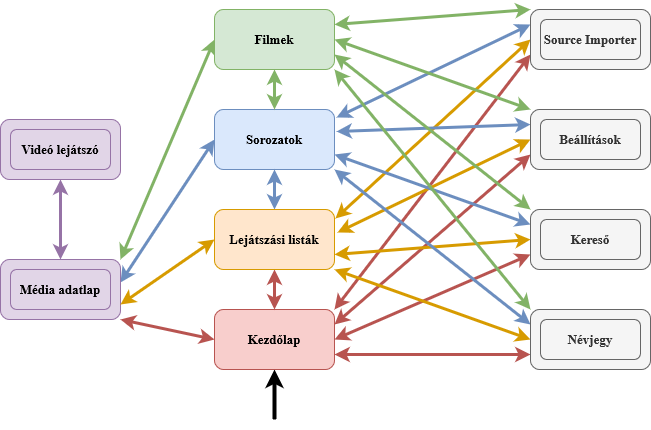
\includegraphics[width=1\textwidth]{navigation_between_screens.png}
	\caption{Navigáció az oldalak között}
	\label{fig:navigation_between_screens}
\end{figure}

% ==========================================================
% |         Hibás vagy eredménytelen megközelítések        |
% ==========================================================
\subsection{Hibás vagy eredménytelen megközelítések}
A program fejlesztésekor számos alkalommal adódtak implementációs nehézségek, amelyek megoldására az eredeti terv kisebb változtatására vagy kiegészítésére volt szükség.

\subsubsection{Korlátozott belső videólejátszó}
Az Electron, ahogy azt már tárgyaltuk, webes technológiákat biztosít asztali alkalmazás fejlesztésre, és ennek korlátozottságaival számolnunk kell. A videólejátszó nem képes minden formátumot lejátszani, ez a HTML <video> tag korlátozottságának tudható be, web által támogatott formátumokon ({\it mp4, webm, vtt}) kívül legtöbb esetben sikeresen lejátssza például az {\it mkv} konténer formátumot is, azonban bizonyos esetekben nincs hang - ez megint csak nem támogatott audió kodek miatt lehetséges - vagy a lejátszásra se képes. Az {\it avi} videóformátumokat viszont egyáltalán nem támogatja a belső lejátszó.
További probléma, amely az eredeti tervtől való kisebb eltérésre kényszerített, a belső videó lejátszó továbbá nem képes a videófájlokba égetett feliratok vagy nyelvek észlelésére és annak változtatására a már fent ismertetett okok miatt.

Ezen probléma megoldására implementálva lett a média tartalom külső videó lejátszóban való megnyitása.

% ==========================================================
% |                      Tesztelés                         |
% ==========================================================
% \cleardoublepage
\section{Tesztelés}
A fejlesztés a legelejétől kezdve gyakorlatilag folyamatos kézi tesztelés mellett zajlott. Erre egy saját automatikusan média tartalmat generáló script került megírásra, amely legenerál egy előre megadott string tömb alapján a videófájlokat, feliratfájlokat és NFO fájlokat egyaránt. Az NFO fájlokba valid IMDB linkeket és TinyURL linekeket generál, a feliratfájlokba - merthogy a script random számú, több formátumú feliratot generál minden videó fájl mellé - továbbá egy rövid szöveget. Fontos megjegyezni, hogy a legenerált videófájlok természetesen nem valós, tört vagy hamis fájlok lesznek, a videó lejátszó nem lesz képes őket lejátszani, de a Scannelés szempontjából tökéletesen megfelelő lesz nekünk teszteléshez.

A tesztfájlok generálásához az alábbi yarn parancsot lehet használni:
\lstset{caption={Teszt fájlok generálása}, label=src:cmd}
\begin{lstlisting}[language={cmd}, numbers={none}]
    yarn generate-media
\end{lstlisting}

\subsection{Scannelés}
A tesztelés legfontosabb része természetesen az Offline és Online Scanneléshez köthető, tekintve ez a program egyik legfontosabb alkotó eleme. Az alábbiakban a scannelés hatékonyságát, sebességét vizsgáljuk.

\begin{figure}[H]
	\centering
	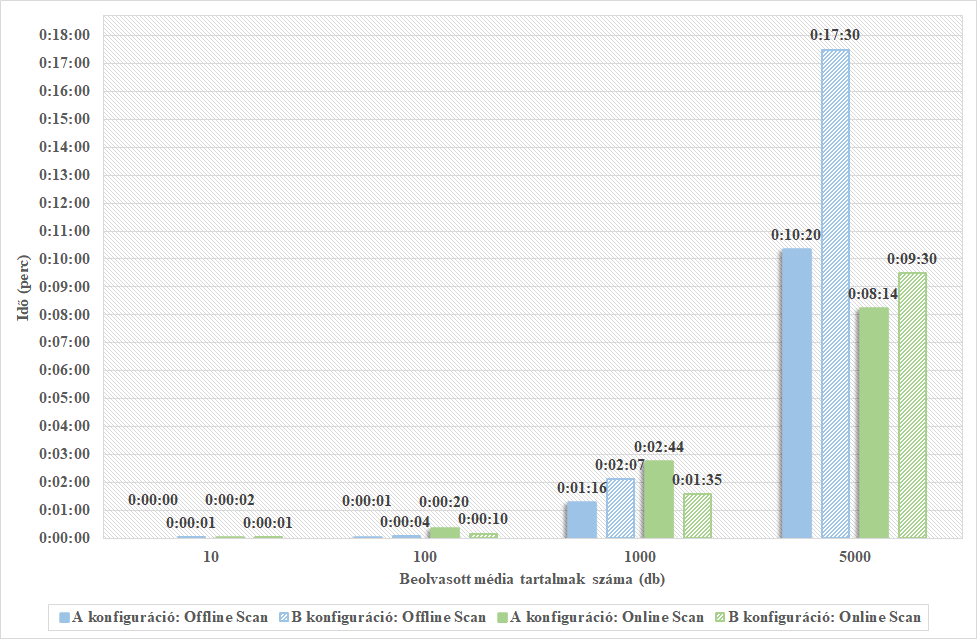
\includegraphics[width=1\textwidth]{scan_time.png}
	\caption{Scannelés időtartamai}
	\label{fig:scan_time}
\end{figure}

{\noindent Az {\textbf A konfiguráció} (Teli oszlopok):}
\begin{itemize}
    \item {\textbf {Processzor: }} AMD Ryzen 7 4800H with Radeon Graphics, 2.90 GHz
    \item {\textbf {Memória: }} 32 GB
    \item {\textbf {Háttértár: }} 500 GB SSD
    \item {\textbf {Operációs rendszer: }} Microsoft Windows 10
\end{itemize}
A {\textbf B konfiguráció} (Csíkos oszlopok):
\begin{itemize}
    \item {\textbf {Processzor: }} Intel Celeron N3350, 1.10 GHz
    \item {\textbf {Memória: }} 4 GB
    \item {\textbf {Háttértár: }} 250 GB SSD
    \item {\textbf {Operációs rendszer: }} Microsoft Windows 10
\end{itemize}

A 3.5 ábráról leolvasható, hogy 10 és 100 média tartalom beolvasása másodpercek vagy tört másodpercek kérdése. 1 000 média tartalom körül lépünk az egy-két perces tartományba, míg 5 000 tartalom esetén tíz-húsz perces tartományba. A két konfiguráció közötti különbség se elhanyagolható, a 10, 100 és 1 000 filmnél még alacsony, de már megfigyelhető különbségek, 5 000 ezer média tartalomnál már viszont szignifikáns különbséget lehet érezni az Offline Scannelés terén, ez a két konfiguráció számítási teljesítményének különbségével magyarázható. Az Online Scannelésnél viszont már nem figyelhető meg olyan számottevő különbség, sőt előfordul, hogy a gyengébb konfigurációjú gépen több ideig tart a Scannelés. Ennek oka az, hogy mindkét gép ugyanarra a hálózatra - ugyanolyan sávszélességel - volt csatolva tesztelés során, tehát az eredmények ezért hasonlóak.
Ezek a számok sokmindent elmondanak az alkalmazás hatékonyságáról és sebességéről, azonban ki kell térni a reális, mindennapi használatra is. A valóságban már 1000 média tartalom is egy elég nagy adattömeg, ha az egyszerűség kedvéért egy filmet 1 gigabájtosnak veszünk, 1000 film tárolására egy egy terrabájtos tárhelyre van szükség, ötezer film tárolása esetén pedig ez a szám már 5 TB. Ha a valóság irányába mégnagyobb gesztust szeretnénk tenni, az 1 film - 1 GB egyszerűsítés nem állja ki a próbát, ugyanis ma már egy gyengébb minőségű film is minimum 2-3 GB, a HD filmek pedig 8-10 GB között tendálnak és még ezt is meg lehet fejelni a BluRay vagy UHD filmekkel amelyek 40-50 vagy akár 100 gigabájtot is elérhetik, ha így számolunk már 1 000 film tárolására is több tíz terrabájtos tárhelyre lenne szükség.

Az alkalmazás 10 000 film beolvasásával is tesztelve lett, a beolvasási idő kicsit több mint fél óráig, a metaadatok letöltése pedig kicsit több mint tizenöt percig tartott. A program mindeközben stabilan működött, és le tudta kezelni ezt a nagy mennyiségű beolvasást, majd ezen tartalmak közötti böngészést is.

\cleardoublepage
\subsection{Felhasználói felület tesztelése}
A felhasználó felületet a használati esetek diagram alapján teszteltük manuálisan.

\begin{center}
	\begin{longtable}{ | p{0.3\textwidth} | p{0.7\textwidth} | }

		\hline
		\multicolumn{2}{|c|}{\textbf{Teszt esetek}}
		\\ \hline

		\textbf{Művelet} & \textbf{Várt eredmény}
		\\ \hline \hline
		\endfirsthead % első oldal fejléce

		\hline
		\textbf{Művelet} & \textbf{Várt eredmény}
		\\ \hline \hline
		\endhead % többi oldal fejléce

		\hline
		\endfoot % többi oldal lábléce

		\endlastfoot % utolsó oldal lábléce

		\emph{Menüpontokra kattintás}
		& Az adott menüpontokra kattintás esetén a megfelelő tartalmak jelennek meg vagy a főablakban (például Kezdőlap, Filmek, Sorozatok, Lejátszási listák menüpontok esetén) vagy a megfelelő modal ablak nyílik meg (például Source Importer, Beállítások, Média Adatlap).
		\\ \hline

		\emph{Keresőre kattintás}
		& A keresőre kattintás esetén megnyílik egy legördülő menü, amely az összes beolvasott filmet, sorozatot tartalmazza, amennyiben nincs beolvasott tartalom a kereső jelzi azt.
		\\ \hline

        \emph{Menü ikon}
		& A hamburger ikonra kattintva a menü kinyílik vagy visszazáródik.
		\\ \hline

        \emph{Lejátszási listák létrehozása}
		& A menüsorban a Lejátszási listák ikonra kattintva megnyílik az kis ablak amely a már létező lejátszási listákat tartalmazza - amennyiben nincs ilyen a lista üres -, hozzáadni a lista alján ha beírunk egy nevet és Entert nyomunk vagy a + ikonra kattintunk, a lejátszási lista létrejön.
		\\ \hline

        \emph{Média kártyák listázása}
		& A Kezdőlapon vagy valamelyik tematikus oldalon alapértelemzetten 10 kártya jelenik meg. Ezt az oldal tetején vagy alján a legördülő menüben egy másik számra kattintva megváltozik, 25, 50 vagy 100 filmre/oldal. Az előre és tovább gombokra kattintva lapozni kezd a filmek között.
		\\ \hline

		\emph{Mappák kiválasztása}
		& A Source Improrteren belül a Mappák kiválasztása gombra kattintva, az operációs rendszer párbeszédablaka megnyílik, kiválasztás után a jelölt mappák megjelennek a felületen.
		\\ \hline

        \emph{Mappák törlése}
		& A Source Improrteren belül az Összes mappa törlése gombra kattintva, a mappák törlődnek, míg a kuka ikonra kattintva csak az adott mappa kerül törlésre. Amennyiben nincs kiválasztott mappa a felület nem engedi tovább a felhasználót.
		\\ \hline

        \emph{Offline Scan}
		& A Source Improrteren belül az Offline Scan gombra kattintva a beolvasás elindul, majd lefutást követően a háttérben megjelennek a filmek a felület pedig tovább engedi a felhasználót.
		\\ \hline

        \emph{Online Scan}
		& A Source Improrteren belül az Online Scan gombra kattintva a metaadatok letöltése elindul, befejezést követően a felület tovább enged. Internetkapcsolat hiányában a metadatok letöltése nem lehetséges, ezt a program jelzi is a felhasználó felé.
		\\ \hline

        \emph{Adatbázis kiürítése}
		& A Beállításokon belül az Összes média törlése gombra kattintva, egy párbeszéd ablak nyílik meg, amennyiben a válasz beleegyező volt az összes média törlésre kerül, amennyiben a válasz elutasító volt nem történik semmi.
		\\ \hline

        \emph{Fejlesztői konzol megnyitása}
		& A Beállításokon belül az Fejlesztői konzol megnyitása gombra kattintva, megnyílik a fejlesztői konzol.
		\\ \hline

        \emph{Média adatlap megnyitása}
		& A Kezdőlapon vagy valamelyik tematikus oldalon egy média kártyára kattintva megnyílik annak adatlapja. Az adatlap tartalmazza a beolvasott információkat.
		\\ \hline

        \emph{Média törlése}
		& Az adatlapon, az ikonsorban a Kuka ikonra kattintva, egy párbeszéd ablak nyílik meg, amennyiben a válasz beleegyező volt úgy a média törlése kerül, amennyiben a válasz elutasító volt nem történik semmi.
		\\ \hline

        \emph{IMDB megnyitása}
		& Az adatlapon, az ikonsorban a IMDB ikonra kattintva, megnyíilik a film IMDB adatlapja az alapértelmezett böngészőben. Ha a program nem talált IMDB azonosítót akkor ez a gomb le van tiltva.
		\\ \hline

        \emph{Lejátszási listához adás}
		& Az adatlapon, az ikonsorban az Lejátszási listához adás ikonra kattintva, megjelennek a létező lejátszási listák, a listaikonra rákattintva a film hozzáadódik, az X ikonra kattintva a film törlődik a listából. Amennyiben nincs létező lejátszási lista az ikonra rákattintva ezt jelzi az alkalmazás.
		\\ \hline

        \emph{Borító cseréje}
		& Az adatlapon, az ikonsorban az Üres négyzet ikonra kattintva, amennyiben nincs a filmnek borítóképe úgy megnyíilik az operációs rendszer párbeszédablakja, amennyiben már van borítókép beállítva abban az esetben a borítókép törlődik az ikon pedig egy kereső ikonos kép ikonra módosul.
		\\ \hline

        \emph{Külső lejátszó megnyitása}
		& Az adatlapon a baloldali kis lejátszás ikonra kattintva megnyíilik az adott média az operációs rendszer szerint alapértelmezett külső lejátszóban.
		\\ \hline

        \emph{Belső lejátszó megnyitása}
		& Az adatlapon a lista elemre kattintva megnyíilik az adott média a program belső lejátszójában.
		\\ \hline

		\caption{A felhasználói felület tesztjei}
		\label{tab:ui_tests}
	\end{longtable}
\end{center}

\cleardoublepage

\chapter{Összegzés} % Conclusion
\label{ch:sum}

Az alkalmazás tehát filmek és sorozatok vizualizációját tűzte ki célul, egy jól átlátható, egyszerű felületet a média tartalmaink megtekintésére, belső és külső lejátszóban egyaránt, továbbá listázó plaformként nagyobb filmes kollekciókat egy sokkal látványosabb környezetben tudjuk szemlélni, mintha csak simán a Windows Fájlkezelőben böngészgetnénk, köszönhető ez a tartalmainkhoz metaadatokat be- és letöltő funkciónak is.

A program megalkotása során rengeteget tanultam és tapasztaltam, a számomra eddig idegen és elég kaotikus Node-TypeScript-Electron-React világot már sokkal közelebbinek érzem és átlátom annak működését. Nagyobb projekt megvalósításaként olyan készségeket szereztem, amelyek elengedhetetlenek minden programtervező informatikus számára.

Hosszútávó céljaim az alkalmazással számosak, szeretném továbbfejleszteni közösségi open-source projektként

\cleardoublepage

% MINTA
% \chapter{MINTA Bevezetés} % Introduction
\label{ch:intro}

Lorem ipsum dolor sit amet, consectetur adipiscing elit. In eu egestas mauris. Quisque nisl elit, varius in erat eu, dictum commodo lorem. Sed commodo libero et sem laoreet consectetur. Fusce ligula arcu, vestibulum et sodales vel, venenatis at velit \cite{dahl1972structured}. Aliquam erat volutpat. Proin condimentum accumsan velit id hendrerit. Cras egestas arcu quis felis placerat, ut sodales velit malesuada. Maecenas et turpis eu turpis placerat euismod.\footnote{Maecenas a urna viverra, scelerisque nibh ut, malesuada ex.}

Aliquam suscipit dignissim tempor. Praesent tortor libero, feugiat et tellus porttitor, malesuada eleifend felis. Orci varius natoque penatibus et magnis dis parturient montes, nascetur ridiculus mus \cite{cormen2009algorithms,krasner1988mvc}. Nullam eleifend imperdiet lorem, sit amet imperdiet metus pellentesque vitae. Donec nec ligula urna. Aliquam bibendum tempor diam, sed lacinia eros dapibus id. Donec sed vehicula turpis. Aliquam hendrerit sed nulla vitae convallis. Etiam libero quam, pharetra ac est nec, sodales placerat augue. \citeauthor{dijkstra1979goto} praesent eu consequat purus \cite{dijkstra1979goto}.

% \cleardoublepage
%
% \chapter{MINTA Felhasználói dokumentáció} % User guide
\label{ch:user}

Lorem ipsum dolor sit amet $\mathbb{N}$\nomenclature{$\mathbb{N}$}{Set of natural numbers}, consectetur adipiscing elit. Duis nibh leo, dapibus in elementum nec, aliquet id sem. Suspendisse potenti. Nullam sit amet consectetur nibh. Donec scelerisque varius turpis at tincidunt. Cras a diam in mauris viverra vehicula. Vivamus mi odio, fermentum vel arcu efficitur, lacinia viverra nibh. Aliquam aliquam ante mi, vel pretium arcu dapibus eu. Nulla finibus ante vel arcu tincidunt, ut consectetur ligula finibus. Mauris mollis lectus sed ipsum bibendum, ac ultrices erat dictum. Suspendisse faucibus euismod lacinia $\mathbb{Z}$\nomenclature{$\mathbb{Z}$}{Set of integer numbers}.


\section{MINTA Felsorolások} % Enumerations and lists

Etiam vel odio ante. Etiam pulvinar nibh quis massa auctor congue. Pellentesque quis odio vitae sapien molestie vestibulum sit amet et quam. Pellentesque vel dui eget enim hendrerit finibus at sit amet libero. Quisque sollicitudin ultrices enim, nec porta magna imperdiet vitae. Cras condimentum nunc dui, eget molestie nunc accumsan vel.

\begin{itemize}
	\item Fusce in aliquet neque, in pretium sem.
	\item Donec tincidunt tellus id lectus pretium fringilla.
	\item Nunc faucibus, erat pretium tempus tempor, tortor mi fringilla neque, ac congue ex dui vitae mauris.
\end{itemize}

Donec dapibus sodales ante, at scelerisque nunc laoreet sit amet. Mauris porttitor tincidunt neque, vel ullamcorper neque pulvinar et. Integer eu lorem euismod, faucibus lectus sed, accumsan felis. Nunc ornare mi at augue vulputate, eu venenatis magna mollis. Nunc sed posuere dui, et varius nulla. Sed mollis nibh augue, eget scelerisque eros ornare nec.

\begin{enumerate}
	\item\label{step:first} Donec pretium et quam a cursus. Ut sollicitudin tempus urna et mollis.
	\item Aliquam et aliquam turpis, sed fermentum mauris. Nulla eget ex diam.
	\item Donec eget tellus pharetra, semper neque eget, rutrum diam Step~\ref{step:first}.
\end{enumerate}

Praesent porta, metus eget eleifend consequat, eros ligula eleifend ex, a pellentesque mi est vitae urna. Vivamus turpis nunc, iaculis non leo eget, mattis vulputate tellus. Maecenas rutrum eros sem, pharetra interdum nulla porttitor sit amet. In vitae viverra ante. Maecenas sit amet placerat orci, sed tincidunt velit. Vivamus mattis, enim vel suscipit elementum, quam odio venenatis elit\footnote{Phasellus faucibus varius purus, nec tristique enim porta vitae.}, et mollis nulla nunc a risus. Praesent purus magna, tristique sed lacus sit amet, convallis malesuada magna.

\begin{description}
	\item[Vestibulum venenatis] malesuada enim, ac auctor erat vestibulum et. Phasellus id purus a leo suscipit accumsan.
	\item[Orci varius natoque] penatibus et magnis dis parturient montes, nascetur ridiculus mus. Nullam interdum rhoncus nisl, vel pharetra arcu euismod sagittis. Vestibulum ac turpis auctor, viverra turpis at, tempus tellus.
	\item[Morbi dignissim] erat ut rutrum aliquet. Nulla eu rutrum urna. Integer non urna at mauris scelerisque rutrum sed non turpis.
\end{description}

\subsection{Szoros térközű felsorolások} % Lists with narrow spacing inbetween items

Phasellus ultricies, sapien sit amet ultricies placerat, velit purus viverra ligula, id consequat ipsum odio imperdiet enim:
\begin{compactenum}
	\item Maecenas eget lobortis leo.
	\item Donec eget libero enim.
	\item In eu eros a eros lacinia maximus ullamcorper eget augue.
\end{compactenum}

\bigskip

In quis turpis metus. Proin maximus nibh et massa eleifend, a feugiat augue porta. Sed eget est purus. Duis in placerat leo. Donec pharetra eros nec enim convallis:
\begin{compactitem}
	\item Pellentesque odio lacus.
	\item Maximus ut nisl auctor.
	\item Sagittis vulputate lorem.
\end{compactitem}

\bigskip

Vestibulum ante ipsum primis in faucibus orci luctus et ultrices posuere cubilia Curae; Sed lorem libero, dignissim vitae gravida a, ornare vitae est.
\begin{compactdesc}
	\item[Cras maximus] massa commodo pellentesque viverra.
	\item[Morbi sit] amet ante risus. Aliquam nec sollicitudin mauris
	\item[Ut aliquam rhoncus sapien] luctus viverra arcu iaculis posuere
\end{compactdesc}


\section{MINTA Képek, ábrák} % Images and figures

Aliquam vehicula luctus mi a pretium. Nulla quam neque, maximus nec velit in, aliquam mollis tortor. Aliquam erat volutpat. Curabitur vitae laoreet turpis. Integer id diam ligula. Nulla sodales purus id mi consequat, eu venenatis odio pharetra. Cras a arcu quam. Suspendisse augue risus, pulvinar a turpis et, commodo aliquet turpis. Nulla aliquam scelerisque mi eget pharetra. Mauris sed posuere elit, ac lobortis metus. Proin lacinia sit amet diam sed auctor. Nam viverra orci id sapien sollicitudin, a aliquam lacus suscipit, Figure~\ref{fig:example-1}:

\begin{figure}[H]
	\centering
	\includegraphics[width=0.6\textwidth,height=100px]{elte_cimer/elte_cimer_szines}
	\caption{Quisque ac tincidunt leo}
	\label{fig:example-1}
\end{figure}

\subsection{Képek szegélyezése} % Framing figures

Ut aliquet nec neque eget fermentum. Cras volutpat tellus sed placerat elementum. Quisque neque dui, consectetur nec finibus eget, blandit id purus. Nam eget ipsum non nunc placerat interdum.

\begin{figure}[H]
	\centering
	\includegraphics[width=0.6\textwidth,height=100px,frame]{elte_cimer/elte_cimer_szines}
	\caption{Quisque ac tincidunt leo}
\end{figure}

\subsection{Képek csoportosítása} % Subfigures

In non ipsum fermentum urna feugiat rutrum a at odio. Pellentesque habitant morbi tristique senectus et netus et malesuada fames ac turpis egestas. Nulla tincidunt mattis nisl id suscipit. Sed bibendum ac felis sed volutpat. Nam pharetra nisi nec facilisis faucibus. Aenean tristique nec libero non commodo. Nulla egestas laoreet tempus. Nunc eu aliquet nulla, quis vehicula dui. Proin ac risus sodales, gravida nisi vitae, efficitur neque, Figure~\ref{fig:example-2}:

\begin{figure}[H]
	\centering
	\subfigure[Vestibulum quis mattis urna]{
		\includegraphics[width=0.45\linewidth]{elte_cimer/elte_cimer_szines}}
	\hspace{5pt}
	\subfigure[Donec hendrerit quis dui sit amet venenatis]{
		\includegraphics[width=0.45\linewidth]{elte_cimer/elte_cimer_szines}}
	\caption{Aenean porttitor mi volutpat massa gravida}
	\label{fig:example-2}
\end{figure}

Nam et nunc eget elit tincidunt sollicitudin. Quisque ligula ipsum, tempor vitae tortor ut, commodo rhoncus diam. Pellentesque habitant morbi tristique senectus et netus et malesuada fames ac turpis egestas. Phasellus vehicula quam dui, eu convallis metus porta ac.


\section{MINTA Táblázatok} % Tables

Nam magna ex, euismod nec interdum sed, sagittis nec leo. Nam blandit massa bibendum mattis tristique. Phasellus tortor ligula, sodales a consectetur vitae, placerat vitae dolor. Aenean consequat in quam ac mollis.

\begin{table}[H]
	\centering
	\begin{tabular}{ | m{0.25\textwidth} | m{0.65\textwidth} | }
		\hline
		\textbf{Phasellus tortor} & \textbf{Aenean consequat} \\
		\hline \hline
		\emph{Sed malesuada} & Aliquam aliquam velit in convallis ultrices. \\
		\hline
		\emph{Purus sagittis} &  Quisque lobortis eros vitae urna lacinia euismod. \\
		\hline
		\emph{Pellentesque} & Curabitur ac lacus pellentesque, eleifend sem ut, placerat enim. Ut auctor tempor odio ut dapibus. \\
		\hline
	\end{tabular}
	\caption{Maecenas tincidunt non justo quis accumsan}
	\label{tab:example-1}
\end{table}

\subsection{Sorok és oszlopok egyesítése} % Multi rows and multi columns

Mauris a dapibus lectus. Vestibulum commodo nibh ante, ut maximus magna eleifend vel. Integer vehicula elit non lacus lacinia, vitae porttitor dolor ultrices. Vivamus gravida faucibus efficitur. Ut non erat quis arcu vehicula lacinia. Nulla felis mauris, laoreet sed malesuada in, euismod et lacus. Aenean at finibus ipsum. Pellentesque dignissim elit sit amet lacus congue vulputate.

\begin{table}[htb]
	\centering
	\begin{tabular}{ | c | r | r | r | r | r | r | }
		\hline
		\multirow{2}{*}{\textbf{Quisque}} & \multicolumn{2}{ c | }{\textbf{Suspendisse}} & \multicolumn{2}{ c | }{\textbf{Aliquam}} & \multicolumn{2}{ c | }{\textbf{Vivamus}} \\
		\cline{2-7}
		& Proin & Nunc & Proin & Nunc & Proin & Nunc \\
		\hline \hline
		Leo & 2,80 MB & 100\% & 232 KB & 8,09\% & 248 KB & 8,64\% \\
		\hline
		Vel & 9,60 MB & 100\% & 564 KB & 5,74\% & 292 KB & 2,97\% \\
		\hline
		Auge & 78,2 MB & 100\% & 52,3 MB & 66,88\% & 3,22 MB & 4,12\% \\
		\hline
	\end{tabular}
	\caption[Rövid cím a táblázatjegyzékbe]{Vivamus ac arcu fringilla, fermentum neque sed, interdum erat. Mauris bibendum mauris vitae enim mollis, et eleifend turpis aliquet.}
	\label{tab:example-2}
\end{table}

\subsection{Több oldalra átnyúló táblázatok} % Long tables over multiple pages

Nunc porta placerat leo, sit amet porttitor dui porta molestie. Aliquam at fermentum mi. Maecenas vitae lorem at leo tincidunt volutpat at nec tortor. Vivamus semper lacus eu diam laoreet congue. Vivamus in ipsum risus. Nulla ullamcorper finibus mauris non aliquet. Vivamus elementum rhoncus ex ut porttitor.

\begin{center}
	\begin{longtable}{ | p{0.3\textwidth} | p{0.7\textwidth} | }

		\hline
		\multicolumn{2}{|c|}{\textbf{Praesent aliquam mauris enim}}
		\\ \hline

		\emph{Suspendisse potenti} & \emph{Lorem ipsum dolor sit amet}
		\\ \hline \hline
		\endfirsthead % első oldal fejléce

		\hline
		\emph{Suspendisse potenti} & \emph{Lorem ipsum dolor sit amet}
		\\ \hline \hline
		\endhead % többi oldal fejléce

		\hline
		\endfoot % többi oldal lábléce

		\endlastfoot % utolsó oldal lábléce

		\emph{Praesent}
		& Nulla ultrices et libero sit amet fringilla. Nunc scelerisque ante tempus sapien placerat convallis.
		\\ \hline

		\emph{Luctus}
		& Integer hendrerit erat massa, non hendrerit risus convallis at. Curabitur ultrices, justo in imperdiet condimentum, neque tortor luctus enim, luctus posuere massa erat vitae nibh.
		\\ \hline

		\emph{Egestas}
		& Duis fermentum feugiat augue in blandit. Mauris a tempor felis. Pellentesque ultricies tristique dignissim. Pellentesque aliquam semper tristique. Nam nec egestas dolor. Vestibulum id elit quis enim fringilla tempor eu a mauris. Aliquam vitae lacus tellus. Phasellus mauris lectus, aliquam id leo eget, auctor dapibus magna. Fusce lacinia felis ac elit luctus luctus.
		\\ \hline

		\emph{Dignissim}
		& Praesent aliquam mauris enim, vestibulum posuere massa facilisis in. Suspendisse potenti. Nam quam purus, rutrum eu augue ut, varius vehicula tellus. Fusce dui diam, aliquet sit amet eros at, sollicitudin facilisis quam. Phasellus tempor metus vel augue gravida pretium. Proin aliquam aliquam blandit. Nulla id tempus mi. Fusce in aliquam tortor.
		\\ \hline

		\emph{Pellentesque}
		& Donec felis nibh, imperdiet a arcu non, vehicula gravida nibh. Quisque interdum sapien eu massa commodo, ac elementum felis faucibus.
		\\ \hline

		\emph{Molestie}
		& Cras ullamcorper tellus et auctor ultricies. Maecenas tincidunt euismod lectus nec venenatis. Suspendisse potenti. Pellentesque pretium nunc ut euismod cursus. Nam venenatis condimentum quam. Curabitur suscipit efficitur aliquet. Interdum et malesuada fames ac ante ipsum primis in faucibus.
		\\ \hline

		\emph{Vivamus semper}
		& In purus purus, faucibus eu libero vulputate, tristique sodales nunc. Nulla ut gravida dolor. Fusce vel pellentesque mi, vel efficitur eros. Nunc vitae elit tellus. Sed vestibulum auctor consequat.
		\\ \hline

		\emph{Condimentum}
		& Nulla scelerisque, leo et facilisis pretium, risus enim cursus turpis, eu suscipit ipsum ipsum in mauris. Praesent eget pulvinar ipsum, suscipit interdum nunc. Nam varius massa ut justo ullamcorper sollicitudin. Vivamus facilisis suscipit neque, eu fermentum risus. Ut at mi mauris.
		\\ \hline

		\caption{Praesent ullamcorper consequat tellus ut eleifend}
		\label{tab:example-3}
	\end{longtable}
\end{center}

% \cleardoublepage
%
% \chapter{MINTA Fejlesztői dokumentáció} % Developer guide
\label{ch:impl}

Lorem ipsum dolor sit amet, consectetur adipiscing elit. Duis nibh leo, dapibus in elementum nec, aliquet id sem. Suspendisse potenti. Nullam sit amet consectetur nibh. Donec scelerisque varius turpis at tincidunt.


\section{MINTA Tételek, definíciók, megjegyzések} % Theorem-like items

\begin{definition}
Mauris tristique sollicitudin ultrices. Etiam tristique quam sit amet metus dictum imperdiet. Nunc id lorem sed nisl pulvinar aliquet vitae quis arcu. Morbi iaculis eleifend porttitor.
\end{definition}

Maecenas rutrum eros sem, pharetra interdum nulla porttitor sit amet. In vitae viverra ante. Maecenas sit amet placerat orci, sed tincidunt velit. Vivamus mattis, enim vel suscipit elementum, quam odio venenatis elit, et mollis nulla nunc a risus. Praesent purus magna, tristique sed lacus sit amet, convallis malesuada magna. Phasellus faucibus varius purus, nec tristique enim porta vitae.

\begin{theorem}
Nulla finibus ante vel arcu tincidunt, ut consectetur ligula finibus. Mauris mollis lectus sed ipsum bibendum, ac ultrices erat dictum. Suspendisse faucibus euismod lacinia. Etiam vel odio ante.
\end{theorem}
\begin{proof}
Etiam pulvinar nibh quis massa auctor congue. Pellentesque quis odio vitae sapien molestie vestibulum sit amet et quam. Pellentesque vel dui eget enim hendrerit finibus at sit amet libero. Quisque sollicitudin ultrices enim, nec porta magna imperdiet vitae. Cras condimentum nunc dui.
\end{proof}

Donec dapibus sodales ante, at scelerisque nunc laoreet sit amet. Mauris porttitor tincidunt neque, vel ullamcorper neque pulvinar et. Integer eu lorem euismod, faucibus lectus sed, accumsan felis.

\begin{remark}
Nunc ornare mi at augue vulputate, eu venenatis magna mollis. Nunc sed posuere dui, et varius nulla. Sed mollis nibh augue, eget scelerisque eros ornare nec. Praesent porta, metus eget eleifend consequat, eros ligula eleifend ex, a pellentesque mi est vitae urna. Vivamus turpis nunc, iaculis non leo eget, mattis vulputate tellus.
\end{remark}

Fusce in aliquet neque, in pretium sem. Donec tincidunt tellus id lectus pretium fringilla. Nunc faucibus, erat pretium tempus tempor, tortor mi fringilla neque, ac congue ex dui vitae mauris. Donec pretium et quam a cursus.

\begin{note}
Aliquam vehicula luctus mi a pretium. Nulla quam neque, maximus nec velit in, aliquam mollis tortor. Aliquam erat volutpat. Curabitur vitae laoreet turpis. Integer id diam ligula.
\end{note}

Ut sollicitudin tempus urna et mollis. Aliquam et aliquam turpis, sed fermentum mauris. Nulla eget ex diam. Donec eget tellus pharetra, semper neque eget, rutrum diam.

\subsection{MINTA Egyenletek, matematika} % Equations, formulas

Duis suscipit ipsum nec urna blandit, $2 + 2 = 4$ pellentesque vehicula quam fringilla. Vivamus euismod, lectus sit amet euismod viverra, dolor metus consequat sapien, ut hendrerit nisl nulla id nisi. Nam in leo eu quam sollicitudin semper a quis velit.

$$a^2 + b^2 = c^2$$

Phasellus mollis, elit sed convallis feugiat, dolor quam dapibus nibh, suscipit consectetur lacus risus quis sem. Vivamus scelerisque porta odio, vitae euismod dolor accumsan ut.

In mathematica, identitatem Euleri (equation est scriptor vti etiam notum) sit aequalitatem Equation~\ref{eq:euler}:
\begin{equation}\label{eq:euler}
e^{i \times \pi} + 1 = 0
\end{equation}


\section{MINTA Forráskódok} % Source code samples

Nulla sodales purus id mi consequat, eu venenatis odio pharetra. Cras a arcu quam. Suspendisse augue risus, pulvinar a turpis et, commodo aliquet turpis. Nulla aliquam scelerisque mi eget pharetra. Mauris sed posuere elit, ac lobortis metus. Proin lacinia sit amet diam sed auctor. Nam viverra orci id sapien sollicitudin, a aliquam lacus suscipit. Quisque ac tincidunt leo Code~\ref{src:cpp} and \ref{src:csharp}:

\lstset{caption={Hello World in C++}, label=src:cpp}
\begin{lstlisting}[language={C++}]
#include <stdio>

int main()
{
	int c;
	std::cout << "Hello World!" << std::endl;

	std::cout << "Press any key to exit." << std::endl;
	std::cin >> c;

	return 0;
}
\end{lstlisting}

\lstset{caption={Hello World in C\#}, label=src:csharp}
\begin{lstlisting}[language={[Sharp]C}]
using System;
namespace HelloWorld
{
	class Hello
	{
		static void Main()
		{
			Console.WriteLine("Hello World!");

			Console.WriteLine("Press any key to exit.");
			Console.ReadKey();
		}
	}
}
\end{lstlisting}

\subsection{MINTA Algoritmusok} % Algorithms

A general Interval Branch and Bound algorithm is shown in Algorithm~\ref{alg:ibb}. One of the following selection rules is applied in Step \ref{step:selrule}.\\
Példa forrása: \href{https://www.inf.u-szeged.hu/actacybernetica/}{Acta Cybernetica (ez egy link)}.

\begin{algorithm}[H]
\caption{A general interval B\&B algorithm}
\label{alg:ibb}
\textbf{\underline{Funct}} IBB($S,f$)
\begin{algorithmic}[1] % sorszámok megjelenítése minden n. sor előtt, most n = 1
\STATE Set the working list ${\cal L}_W$ := $\{S\}$ and the final list ${\cal L}_Q$ := $\{\}$
\WHILE{( ${\cal L}_W \neq \emptyset$ )} \label{alg:igoend}
	\STATE  Select an interval $X$ from ${\cal L}_W$ \label{step:selrule}\COMMENT{Selection rule}
	\STATE Compute $lbf(X)$ \COMMENT{Bounding rule}
	\IF[Elimination rule]{$X$ cannot be eliminated}
		\STATE Divide $X$ into $X^j,\ j=1,\dots, p$, subintervals   \COMMENT{Division rule}
		\FOR{$j=1,\ldots,p$}
			\IF[Termination rule]{$X^j$ satisfies the termination criterion}
				\STATE Store $X^j$ in ${\cal L}_W$
			\ELSE
				\STATE Store $X^j$ in ${\cal L}_W$
			\ENDIF
		\ENDFOR
	\ENDIF
\ENDWHILE
\STATE \textbf{return} ${\cal L}_Q$
\end{algorithmic}
\end{algorithm}

% \cleardoublepage
%
% \chapter{MINTA Összegzés} % Conclusion
\label{ch:sum}

Lorem ipsum dolor sit amet, consectetur adipiscing elit. In eu egestas mauris. Quisque nisl elit, varius in erat eu, dictum commodo lorem. Sed commodo libero et sem laoreet consectetur. Fusce ligula arcu, vestibulum et sodales vel, venenatis at velit. Aliquam erat volutpat. Proin condimentum accumsan velit id hendrerit. Cras egestas arcu quis felis placerat, ut sodales velit malesuada. Maecenas et turpis eu turpis placerat euismod. Maecenas a urna viverra, scelerisque nibh ut, malesuada ex.

Aliquam suscipit dignissim tempor. Praesent tortor libero, feugiat et tellus porttitor, malesuada eleifend felis. Orci varius natoque penatibus et magnis dis parturient montes, nascetur ridiculus mus. Nullam eleifend imperdiet lorem, sit amet imperdiet metus pellentesque vitae. Donec nec ligula urna. Aliquam bibendum tempor diam, sed lacinia eros dapibus id. Donec sed vehicula turpis. Aliquam hendrerit sed nulla vitae convallis. Etiam libero quam, pharetra ac est nec, sodales placerat augue. Praesent eu consequat purus.

% \cleardoublepage

% Függelékek (opcionális) - hosszabb részletező táblázatok, sok és/vagy nagy kép esetén hasznos
% Appendices (optional) - useful for detailed information in long tables, many and/or large figures, etc.
\appendix
\chapter{A továbbfejlesztési lehetőségekről}
\label{appx:further_development}

Lorem ipsum dolor sit amet, consectetur adipiscing elit. Pellentesque facilisis in nibh auctor molestie. Donec porta tortor mauris. Cras in lacus in purus ultricies blandit. Proin dolor erat, pulvinar posuere orci ac, eleifend ultrices libero. Donec elementum et elit a ullamcorper. Nunc tincidunt, lorem et consectetur tincidunt, ante sapien scelerisque neque, eu bibendum felis augue non est. Maecenas nibh arcu, ultrices et libero id, egestas tempus mauris. Etiam iaculis dui nec augue venenatis, fermentum posuere justo congue. Nullam sit amet porttitor sem, at porttitor augue. Proin bibendum justo at ornare efficitur. Donec tempor turpis ligula, vitae viverra felis finibus eu. Curabitur sed libero ac urna condimentum gravida. Donec tincidunt neque sit amet neque luctus auctor vel eget tortor. Integer dignissim, urna ut lobortis volutpat, justo nunc convallis diam, sit amet vulputate erat eros eu velit. Mauris porttitor dictum ante, commodo facilisis ex suscipit sed.

Sed egestas dapibus nisl, vitae fringilla justo. Donec eget condimentum lectus, molestie mattis nunc. Nulla ac faucibus dui. Nullam a congue erat. Ut accumsan sed sapien quis porttitor. Ut pellentesque, est ac posuere pulvinar, tortor mauris fermentum nulla, sit amet fringilla sapien sapien quis velit. Integer accumsan placerat lorem, eu aliquam urna consectetur eget. In ligula orci, dignissim sed consequat ac, porta at metus. Phasellus ipsum tellus, molestie ut lacus tempus, rutrum convallis elit. Suspendisse arcu orci, luctus vitae ultricies quis, bibendum sed elit. Vivamus at sem maximus leo placerat gravida semper vel mi. Etiam hendrerit sed massa ut lacinia. Morbi varius libero odio, sit amet auctor nunc interdum sit amet.

Aenean non mauris accumsan, rutrum nisi non, porttitor enim. Maecenas vel tortor ex. Proin vulputate tellus luctus egestas fermentum. In nec lobortis risus, sit amet tincidunt purus. Nam id turpis venenatis, vehicula nisl sed, ultricies nibh. Suspendisse in libero nec nisi tempor vestibulum. Integer eu dui congue enim venenatis lobortis. Donec sed elementum nunc. Nulla facilisi. Maecenas cursus id lorem et finibus. Sed fermentum molestie erat, nec tempor lorem facilisis cursus. In vel nulla id orci fringilla facilisis. Cras non bibendum odio, ac vestibulum ex. Donec turpis urna, tincidunt ut mi eu, finibus facilisis lorem. Praesent posuere nisl nec dui accumsan, sed interdum odio malesuada.
\cleardoublepage

% Irodalomjegyzék (kötelező)
% Bibliography (mandatory)
% \addcontentsline{toc}{chapter}{\biblabel}
% \printbibliography[title=\biblabel]
% \cleardoublepage

% Ábrajegyzék (opcionális) - 3-5 ábra fölött érdemes
% List of figures (optional) - useful over 3-5 figures
\addcontentsline{toc}{chapter}{\lstfigurelabel}
\listoffigures
\cleardoublepage

% Táblázatjegyzék (opcionális) - 3-5 táblázat fölött érdemes
% List of tables (optional) - useful over 3-5 tables
% \addcontentsline{toc}{chapter}{\lsttablelabel}
% \listoftables
% \cleardoublepage

% Forráskódjegyzék (opcionális) - 3-5 kódpélda fölött érdemes
% List of codes (optional) - useful over 3-5 code samples
\addcontentsline{toc}{chapter}{\lstcodelabel}
\lstlistoflistings
\cleardoublepage

% Jelölésjegyzék (opcionális)
% List of symbols (optional)
%\printnomenclature

\end{document}
